\addcontentsline{toc}{chapter}{Introduzione}
\chapter*{\begin{center}\texttt{Introduzione}\end{center}}
\hrulefill \\
\addcontentsline{toc}{section}{Cos'è Internet?}
\section*{\textcolor{Blue}{Cos'è Internet?}}
\index{Internet} Fondamentalmente è una rete che collega tra loro più unità di calcolo sparse geograficamente. Si tratta di una \index{rete!a comm. di Pacchetto}rete a commutazione di pacchetto (packet-switch network, PSN), in cui più terminali \index{host}\index{End System}(o End System, o Host, insomma qualsiasi tipo di computer che si trova ad un capo estremo della rete, un laptop, uno smartphone, un sensore...) condividono lo stesso cammino di rete o una parte di esso. Torneremo su commutazione di circuito e di pacchetto a breve.\\


 \noindent Normalmente, i terminali non sono collegati tra loro in modo diretto, ma tramite dispositivi di commutazione e instradamento (router)\index{router} che prelevano le informazioni in dei pacchetti e le inoltrano sui link di uscita. Il percorso compiuto dai pacchetti attraverso la rete prende il nome di Route\index{route}, o Path. Letteralmente \textit{percorso}.\\

 \noindent L'accesso dei terminali ad Internet avviene attraverso gli ISP\index{ISP} (Internet Service Provider), aziende di telecomunicazioni come AT\&T o Vodafone, che costuiscono ciascuna una rete di router a cui poter collegare gli access point come la ADSL domestica (che di per sé costituisce una rete, in questo caso domestica, in cui tutti gli Host comunicano tra loro (internamente) e con il resto di internet (esternamente) attraverso quello che comunemente chiamiamo \index{modem}Modem o \index{gateway}Gateway).\\

 \noindent  TCP/IP: insieme di protocolli (spesso si parla di stack TCP/IP, perché sono posti uno sopra l'altro) che gestiscono invio e ricezione di pacchetti in rete.\\

 \noindent \index{intranet}Intranet: è un tipo di rete privata, strutturata similmente alla pubblica Internet.\\

 \noindent \index{protocollo}Protocollo: insieme di regole formalmente descritte al fine di favorire la comunicazione tra una o più entità (è un termine generico che si può applicare anche ad altri contesti, ovviamente in questo caso parliamo di Host o di componenti in grado di comunicare in rete).\\

 \noindent App distribuite: in Internet si lavora tramite app distribuite, i.e. due o più processi che vengono eseguiti in parallelo su macchine diverse e che interagiscono tra loro attraverso Internet. \\

 \noindent Host: termine che si riferisce a dei sistemi periferici che ospitano programmi applicativi come ad esempio web browser; Gli host si suddividono ulteriormente in Client e Server, rispettivamente host che richiedono un serivizio e quelli che lo forniscono. Un singolo host può fungere da client e da server (connessione Peer-to-Peer). \\

\noindent \index{DSL}DSL (Digital Subscriber Line): accesso residenziale a banda larga. \\ 


\addcontentsline{toc}{section}{Stack dei layer di Internet}
\section*{Stack dei layer di Internet: TCP/IP VS modello ISO/OSI}
\index{TCP/IP, stack}\index{ISO/OSI, modello}
\begin{table}[h]
\begin{tabular}{|ll|ll|l}
\cline{1-4}
\multicolumn{2}{|l|}{TCP/IP}            & \multicolumn{2}{l|}{ISO/OSI}                                                                                                                             &                                                                                                      \\ \hline
\multicolumn{1}{|l|}{Layer}        & n° & \multicolumn{1}{l|}{Layer}                                                                           & n°                                                & \multicolumn{1}{l|}{Esempi di Protocolli}                                                            \\ \hline
\multicolumn{1}{|l|}{Applicazione} & 5  & \multicolumn{1}{l|}{\begin{tabular}[c]{@{}l@{}}Applicazione\\ Presentazione\\ Sessione\end{tabular}} & \begin{tabular}[c]{@{}l@{}}7\\ 6\\ 5\end{tabular} & \multicolumn{1}{l|}{\begin{tabular}[c]{@{}l@{}}HTTP(S), POP, SMTP,\\ FTP, SSH, DHCP...\end{tabular}} \\ \hline
\multicolumn{1}{|l|}{Trasporto}    & 4  & \multicolumn{1}{l|}{Trasporto}                                                                       & 4                                                 & \multicolumn{1}{l|}{TCP, UDP}                                                                        \\ \hline
\multicolumn{1}{|l|}{Rete}         & 3  & \multicolumn{1}{l|}{Rete}                                                                            & 3                                                 & \multicolumn{1}{l|}{IPv4, IPv6, ICMP}                                                                      \\ \hline
\multicolumn{1}{|l|}{Datalink}     & 2  & \multicolumn{1}{l|}{Datalink}                                                                        & 2                                                 & \multicolumn{1}{l|}{MAC}                                                                             \\ \hline
\multicolumn{1}{|l|}{Fisico}       & 1  & \multicolumn{1}{l|}{Fisico}                                                                          & 1                                                 & \multicolumn{1}{l|}{Ethernet, cavo coassiale}                                                        \\ \hline
\end{tabular}
\end{table}

 \noindent Sono due rappresentazioni della stessa stack di classi di protocolli, semplicemente l'ISO\footnote{International Standardization Organization, l'agenzia che si occupa di distribuire standard di varie tecnologie e produzioni.} ha separato l'application layer in 3 layers (Application, Presentation, Session), che è una rappresentazione un po' più dettagliata, ma noi faremo riferimento principalmente al modello TCP/IP. (N.B.: alle volte, nel modello TCP/IP, i layer Datalink e Fisico\footnote{il layer fisico/physical alle volte viene detto anche Network Access Layer.} vengono trattati indistintamente, come fossero un layer unico.) \\

\addcontentsline{toc}{section}{Tipi di ritardo e altri concetti}
\section*{Tipi di ritardo e altri concetti}\index{ritardi}
\noindent Tipi di ritardo (accenno, ci torneremo)\footnote{in verità quasi tutto questo capitolo è un accenno a cose che vedremo più avanti in maggiore dettaglio, ndr.} 
\begin{itemize}
    \item [i.] di Elaborazione: si crea nel router per esaminare il pacchetto;
    \item [ii.] di Accodamento: si crea in coda in uscita, un buffer;
    \item [iii.] di Trasmissione $(=\dfrac{L}{R})$: dipende dalla dimensione del pacchetto (L);
    \item[iv.] di Propagazione: prettamente fisico, dipende dalla distanza tra router A e router B.
\end{itemize}

\noindent La somma di questi ritardi costituisce il \index{delay, nodal}nodal delay, il ritardo accumulato ad ogni nodo del percorso. \\

\noindent \index{network!core}\index{network!edge}Network core vs Network edge: fondamentalmente il network edge sono i sistemi periferici (host come laptops o smartphones), mentre il network core è la struttura che li collega (routers etc.). \\

\noindent \index{LAN}LAN (Local Area Network): usata per collegare end systems ad un edge router. La tecnologia d'accesso usata di solito in queste reti è \index{Ethernet}Ethernet. \\

\noindent Standard IEEE che regolamenta il \index{Wi-Fi}Wi-Fi\footnote{Secondo la Wi-Fi Alliance, il termine ``Wi-Fi'' non è mai stato la contrazione di ``\underline{Wi}reless \underline{Fi}delity, sebbene l'IEEE affermi diversamente.}: 802.11. \\

\noindent Qualche nota sui Physical Media (Mezzi di trasmissione fisici, i.e. cavi eccetera):
\begin{itemize}
    \item Twisted Pair Copper wire (il doppino intrecciato in rame)\index{doppino, in rame}:
    \begin{itemize}
        \item UTP\index{UTP} (Unshielded Twisted Pair, doppino non schermato): usato comunemente nelle LAN. Un cavo UTP di categoria 6A può trasmettere ad una velocità fino a 10Gbps;
        \item La ragione per cui i fili nel doppino sono intrecciati a due a due a quella maniera ha a che fare con la cancellazione dei disturbi del segnale;
    \end{itemize}
    \item Cavo coassiale\index{coassiale, cavo}: quello a sezione circolare dell'antenna TV. Può essere usato in contemporanea da più end systems; alcune categorie trasmettono a velocità nell'ordine di diversi Gbps;
    \item Fibra ottica\index{fibra ottica}: molto veloce, molto costosa, va dai 51.8M ai 39.8 Gbps;
\end{itemize}

\noindent \index{tempo di trasmissione}Il tempo di trasmissione è dato da $\dfrac{L}{R}$, dove L = dimensione del pacchetto in bit e R = transmission rate sul link.\\

\noindent \index{Store-and-Forward}Store-and-forward: il router deve ricevere tutto il pacchetto prima di inoltrarlo dove opportuno; così facendo, il ritardo totale diventa $=\dfrac{2L}{R}$ (per ciascun nodo, credo).\\

\noindent \index{modem}``Modem'' sta per \underline{Mo}dulatore-\underline{Dem}odulatore: sebbene spesso ci riferiamo allo ``scatolotto'' che collega la nostra LAN domestica ad Internet con il termine Modem (quei dispositivi come il TIM Hub, insomma, a volte li si chiama anche Router, che non è troppo sbagliato), in realtà il modem è un modulo incluso in quello scatolotto.\\

\noindent \index{rete!a comm. di Pacchetto}Commutazione di Circuito vs Commutazione di Pacchetto\index{rete!a comm. di Circuito}:
\begin{itemize}
    \item Comm. di circuito: le risorse richieste da un end system per comunicare sono riservate ad esso per tutta la durata della connessione; è il caso della telefonia, se qualcuno sta usando il telefono di casa in una stanza, un secondo telefono collegato alla stessa linea non può avviare un'altra chiamata);
    \item Comm. di pacchetto: le risorse non sono riservate, ma più end systems usano il canale più la banda viene limitata a ciascuno;
\end{itemize}

\noindent La commutazione di circuito può avere due tipi di multiplexing\index{multiplexing}: Frequency-division e Time-division:

\begin{figure} [h]
    \centering
    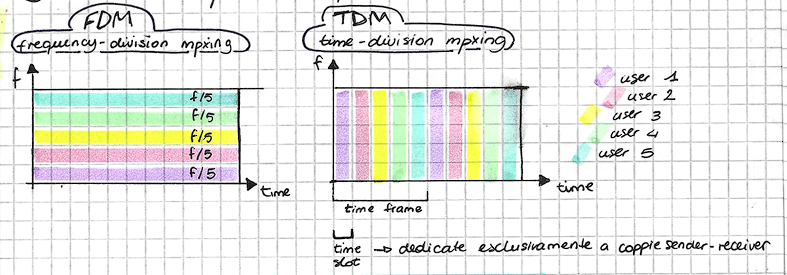
\includegraphics[width=0.6\linewidth]{Figures/01/circswitch.png}
    \label{fig:circswitch}
\end{figure}

\begin{figure}
    \centering
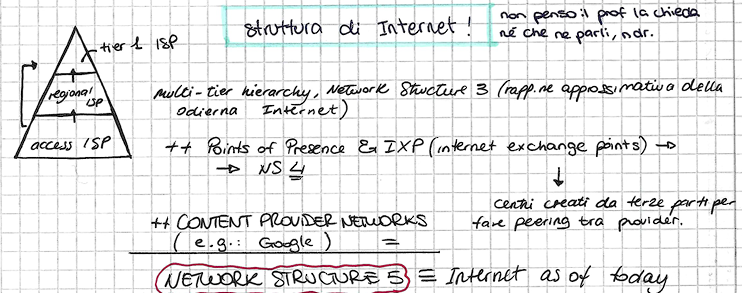
\includegraphics[width=0.8\linewidth]{Figures/01/isp-hierarchy.png}
    \caption{Sì non credo vi verrà richiesta, ma nel dubbio è una cosa del genere.}
    \label{fig:in-structure}
\end{figure}

\noindent In Fig. \ref{fig:in-structure} è riassunta la struttura di Internet e le sue evoluzioni con le varie addizioni di elementi come i Point of Presence \& IXP.\\

\noindent \index{intensità di traffico}Intensità di traffico: $\dfrac{L\cdot a}{R}$, L e R li abbiamo già menzionati, $a=$ average rate of packets per second; un'intensità di traffico $>1$ equivale a dire che la $\#$ di bit che arriva in coda supera la $\#$ di bit che esce dalla coda (converrete con me che è una cosa da evitare, significa che la roba che entra supera la roba che esce, c'è congestione).\\


\begin{wrapfigure}{r}{0.4\textwidth}
 \begin{center}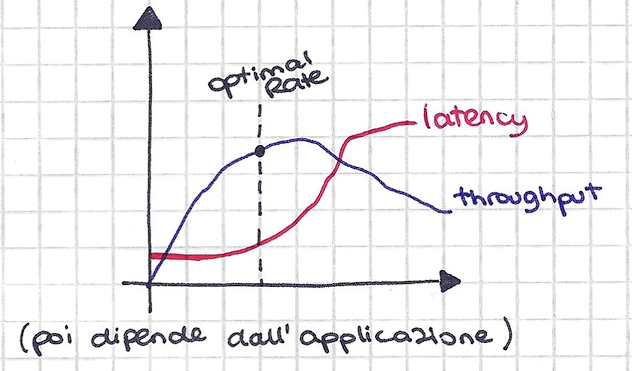
\includegraphics[width=1\linewidth]{Figures//01/optrate.png}
  \end{center}
\end{wrapfigure}
\newpage

\noindent \index{latenza}Latenza: intervallo di tempo tra quando spedisco un input e quando è disponibile l'output.\\

\noindent \index{throughput}Throughput: ``vera velocità'' di rete, vera capacità di un canale trasmissivo. Non si può considerare costante, si parla solo di throughput medio end-to-end.\\

\noindent \index{bandwidth}Bandwidth: intervallo di frequenza che un sistema può garantire per trasmettere. \index{bitrate}Bitrate: dipende dalla bandwidth (teorema di Nyquist-Shannon)\index{teorema!di Shannon}\index{teorema!di Nyquist} (garantito nominalmente).

\begin{figure} [h]
    \centering
    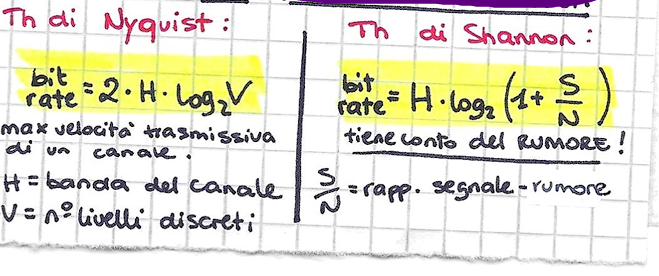
\includegraphics[width=0.5\linewidth]{Figures//01/shannon-nyquist.png}
\end{figure}

\begin{wrapfigure}{l}{0.3\textwidth}
 \begin{center}
 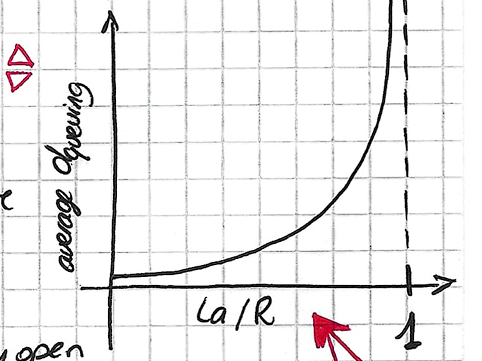
\includegraphics[width=1\linewidth]{Figures/01/laR.png}
  \end{center}
\end{wrapfigure}
\noindent Intensità di traffico: $\dfrac{L\cdot a}{R}$, L e R li abbiamo già menzionati, $a=$ average rate of packets per second; un'intensità di traffico $>1$ equivale a dire che la $\#$ di bit che arriva in coda supera la $\#$ di bit che esce dalla coda (converrete con me che è una cosa da evitare, significa che la roba che entra supera la roba che esce, c'è congestione).\\

\noindent Note sugli attacchi DoS (Denial of Service)\index{attacco!Denial of Service}:
\begin{itemize}
    \item vulnerability attack: usa un messaggio ``maligno'' per compromettere app o host;
\end{itemize}

\begin{itemize}
    \item bandwidth flooding\index{attacco!bandwidth flooding}: invio smisurato di pacchetti al target allo scopo di congestionare l'access link e renderlo inutilizzabile;
    \item \index{attacco!connection flooding}connection flooding: richiesta elevata di connessioni TCP fully open (che rimangono sempre attive) al punto tale che l'host vittima non riesce più ad accettarne altre genuine. Spesso questo attacco è reso possibile grazie a Distributed DoS\index{attacco!DDoS}, i.e. l'attacker controlla più macchine ``zombie''  che dirotta a sua discrezione all'attacco della vittima.
\end{itemize}

\noindent \index{packet sniffing}Packet sniffing (che è quello che fa Wireshark): i bad guys si posizionano tra due host e ``origliano'' il traffico senza manometterlo allo scopo di estrarre informazioni sensibili;

\noindent \index{attacco!IP spoofing}IP spoofing: ``rubare'' l'identità di qualcun altro mediante il suo indirizzo IP;

\noindent \index{traceroute}Traceroute: manda tot pacchetti ai router compresi tra host e destinazione, rilevandoli tutti
\begin{verbatim}
    tracert www.rai.it (212.162.68.64)
\end{verbatim}

\noindent Ogni protocollo appartiene ad un qualche layer della stack e può essere hardware, software o misto.\\

\noindent \index{PDU}PDU (Protocol Data Unit): l'unità di messaggio, che a seconda del layer in cui si trova prende un nome diverso (e.g.: frame, datagramma). La PDU è sempre formata da un header (detto anche PCI o Protocol Control Information) e da un payload (detto anche SDU o Service Data Unit), dove header contiene informazioni per la trasmissione e il payload è il contenuto del messaggio (il payload è generalmente ottenuto dalle PDU dei livelli più alti);

\noindent \index{incapsulamento}Incapsulamento: ciascun layer riceve il messaggio dal layer sopra, aggiunge un suo header, passa il nuovo messaggio al layer sotto. Nel layer sotto succede di nuovo: il layer riceve questo (header + payload) e lo considera come un payload', aggiunge il suo header e passa header' + payload' ancora sotto;\\

\noindent \index{SAP}SAP Service Access Point: servizi messi a disposizione dalle interfacce che si trovano tra due layer comunicanti della stack.\\

\noindent Per fornire accesso a Internet agli utenti, gli ISP distribuiscono lungo il territorio dei PoP, Points of Presence.\\

\noindent Indirizzi della forma $192.168.1.\#\#\#$ non sono indirizzi pubblici, ma interni alla nostra rete.\\

\noindent

\noindent Fiber To The...

\begin{itemize}
    \item FTTH: ...Home
    \item FTTN: ...Node
    \item FTTC: ...Cabinet
    \item FTTS: ...Street (=FTTC)
    \item FTTB: ...Building
\end{itemize}

\noindent \index{best effort}Internet ha un generale approccio al servizio detto ``best effort'' (i.e.: ``che Dio ce la mandi buona''): nulla è di fatto garantito al 100\%, ma tutti fanno del proprio meglio perché funzioni.\\
\newpage
\noindent \index{legge!di Metcalfe}\textcolor{Blue}{Legge di Metcalfe (che allego qui ma non vi serve): ``L'utilità e il valore di una rete sono proporzionali al quadrato del nr di utenti.'' Dato il nr di utenti, il massimo numero di connessioni possibili è $= n^2 - n$. (Si tratta di una legge di dubbia correttezza e largamente contestata, oltre al fatto che non è mai stato possibile testarla con dati reali).}\\

\noindent \textcolor{Blue}{LO! Story Time: La prima parola ad essere trasmessa in una versione preistorica di Internet è stata: \texttt{`LO'}. Transitava dal UCLA al SRI e doveva finire per essere la parola ``LOGIN'', lettera dopo lettera, ma per qualche ragione l'host del SRI crashò ricevendo la G. L'ingegnere Leonard Kleinrock, che era lì a lavorare al progetto ARPANET, scrisse in una celebre intervista che quel tentativo fallito di trasmettere la parola in rete ebbe comunque qualcosa di \textit{profetico:} ``Lo'', come in ``Lo and behold!'' (che più o meno significa \textit{``Ecco, preparatevi!''}), come a presagire la svolta enorme che sarebbe arrivata in futuro dopo quell'esperimento - con la nascita di Internet.}